%start of document preamble
\documentclass[12pt, letterpaper, titlepage]{report}
\usepackage[left=25mm,right=25mm,top=15mm,bottom=15mm]{geometry}
\usepackage[utf8]{inputenc}
\usepackage{natbib}
\usepackage{graphicx}
\usepackage{amsmath}
\usepackage{tikz}
\usepackage{pgfplots}
\setcounter{secnumdepth}{5} % seting level of numbering (default for "report" is 3). With ''-1'' you have non number also for chapters
\setcounter{tocdepth}{5} % if you want all the levels in your table of contents

%\usepackage[english]{babel}
%\usepackage{biblatex}
%\usepackage[style=authoryear]{biblatex}
%\addbibresource{sample.bib}

%end of document preamble

\title{\textbf{Big-data analytics using rules-based techniques and machine learning to support business decisions}}
\author{Joshua Uzochukwu Nwankwo}
%\author{Joshua Uzochukwu Nwankwo \thanks{funded by the ShareLaTeX team}}
\date{April 2018}

\renewcommand*\contentsname{Table of Contents}

\pgfplotsset{width=7cm,compat=1.8}
\pgfmathdeclarefunction{gauss}{2}{%
	\pgfmathparse{1/(#2*sqrt(2*pi))*exp(-((x-#1)^2)/(2*#2^2))}%
}





\begin{document}

\maketitle
\newpage

\begin{abstract}
The following examples show how to produce Harvard style referencing using biblatex.
\end{abstract}

\tableofcontents
\newpage

\chapter{Introduction}
\section{Overview}
\section{Motivation}
\section{Project Objectives}
\section{Thesis organisation}

\chapter{Background}

\chapter{Theoretical and Mathematical Aspects}
\section{Introduction}
\section{Probability and Information Theory}
Machine learning deals with uncertain or stochastic(non-deterministic) quantities. Stochasticity and uncertainty arise from various sources. \cite{goodfellow2016deep} summarised incomplete information about the system being modeled \textbf{incomplete modeling}; the inability to observe all the variables and factors that influence the behaviour of a system \textbf{incomplete observability}; and gaps or unknowns within the system being modeled \textbf{inherent stochasticity} as the three possible sources of uncertainty in machine learning.\\
The goal of machine learning is to predict the chance, likelihood or possibility that an event will occur given that similar events had already occurred. \cite{Murphy2012} described machine learning as a set of methods used to predict future occurrences or used to drive the decision making process where a level of uncertainty exists, uncovering and exploiting patterns in a previously examined event.A mathematical framework for representing, quantifying and deriving uncertainty is known as the probability theory \citep{goodfellow2016deep}  
\section{Z-score Model}
Z-score is the amount or number of standard deviations below or above the mean of a given population or sample. It describes the score of a random variable $X$ relative to the mean and standard deviation.
A basic z-score formula is:

$$z=\dfrac{(datapoint - mean)}{stdev}$$
$$z=\dfrac{(x-\mu)}{\sigma}$$


\subsection{Importance of Z-scores}
\begin{itemize}
	\item It is used to describe how abnormal or normal a situation within a probability distribution are.
	\item It compares the score across different distributions.
	\item It is used to derive the exact location of a score in a probability distribution.
\end{itemize}	
The result of Z-score is signed, positive sign indicates that it is to the right of the mean while a negative sign indicates that it is to the left of the mean.

\subsection{Applications of Z-scores}
Z-scores could be used to derive unknown probabilities from a sample which follows a normal distribution.
For example, we could use the z-score to calculate the probability that the running time of a database query extracted from the log files took over 1 minute(60 seconds). This information would be useful to quantify the percentage of slow-performing queries. \\
\begin{table}[h!]
	\centering
	
	
	\begin{tabular}{|l|l|l|}
		\hline
		\textbf{Mean} & \textbf{Std. Dev} & \textbf{Data Point (Sec)} \\ \hline
		35.51         & 18.21             & 60                        \\ \hline
	\end{tabular}
	\caption{Sample data for z-score computation}
	\label{sampleDataZscore}
\end{table}



$$
P(X>60) = \dfrac{(60-35.51)}{18.21}
        = \dfrac{24.49}{18.21} = 1.35
$$

$1.35$ from the z-score table occupies an area of $0.9115$ which is equivalent to $91.15\%$\\
The total area under the bell-shaped curve is 1 or 100\%, therefore the unknown fragment of the normal distribution is:\\
$$100 - 95.15 = 8.85\%$$

This implies that the probability of a database query taking over 60 seconds is $0.0885$ or $8.85\%$

\section{Machine Learning Algorithms}
\section{K-means Clustering}
\subsection{Euclidean Distance}
\section{Naive Bayes Classifier}
\subsection{Gaussian Naive Bayes}
\subsection{Bernoulli Naive Bayes}
One implementation of the Naive Bayes classifier is the Bernoulli Naive Bayes classifier. It is modeled as a Bernoulli distribution. Bernoulli NB classifier assumes that all the features present in the data frame can be represented as boolean or binary values. Since Bernoulli NB classifier assumes that the data is distributed in accordance to multivariate Bernoulli distribution, this implies that each data point is a binary vector \citep{shimodaira2014text}.\\
In the implementation and methodology section I have discussed how this model has been applied during the data transformation phase. The process basically involves reconstructing the raw data input into a Bernoulli vector. The possible outcome for each data point is denoted as $$x = \{0,1\}$$\\ 

It is worth noting that all Bernoulli distributions are Binomial distributions. In fact Bernoulli distributions are a special case of Binomial distributions where the number of trials $n=1$\\

If
$$
X=\begin{cases} 1 & \text{with probability }p, \\ 0 & \text{with probability }1-p, \end{cases}
$$
then the probability distribution of the random variable $X$ is a Bernoulli distribution.\\

If $X=X_1+\cdots+X_n$ and each of $X_1,\ldots,X_n$ has a Bernoulli distribution with the same value of $p$ and they are independent, then $X$ has a binomial distribution, and the possible values of $X$ are $\{0,1,2,3,\ldots,n\}$.  If $n=1$ then that binomial distribution is a Bernoulli distribution.

\subsubsection*{What is a Bernoulli Random Variable?}
A Bernoulli random variable is one that has one of two possible outcomes.That is, a random variable $X$ is one that satisfies the condition $P(X=1) = p$ or it's complement $P(X=0) = 1 - p$ 

\subsection{Multinomial Naive Bayes}



\section{Decision Trees}
\section{Selection of Features}
\section{Data File Vectorization}
One major challenge with machine learning algorithms is the inability to handle raw textual input. Source files, system, console and web server logs all come in plain text format. They cannot be used in this raw form for analytics and machine learning. Most learning algorithms take input features as numeric vectors. Therefore,conversion of textual documents into vector forms is a required step. The technique used to transform text elements in data sets into numeric vectors is known as \textbf{text vectorization}. Bag-of-words, Boolean Existential and Fuzzy Relevance Matrix are some vectorization models which could be used.
\subsection{Word Count Frequency Approach}
This technique is also known as the \textbf{bag-of-words} model. It involves counting and representing each word in the document as a vector space. A document-term matrix (DTM) is first constructed for each word. Each row in the DTM corresponds to the data file or raw document while each column corresponds to the terms. In text vectorization we often use terms as opposed to words.
\subsection{Boolean Existential Approach}
This model is used to represents each word in the document as a logical or boolean matrix. The raw input is validated using certain rules and criteria, if that condition is met, then the value is set to 1 otherwise it is assigned the default value of 0. Each cell in the matrix can only hold one value which must either be 0 or 1, these are the only possible entries this matrix can hold.
\subsection{Fuzzy Relevance Matrix}

This project adopted  xxxx and xxx vectorization approach 



\section{Summary}



\newpage
\chapter{\textbf{Methodology}}

\section{Introduction}
This chapter details the procedure used to attain the stated objectives. It describes what has been done to address this problems. It starts off by presenting the various machine learning algorithms that were used during the course of this project, it also justifies the rationale behind some of the adopted design decisions. This chapter elucidates the evaluation techniques used to validate the accuracy and correctness of the applied machine learning algorithms.

\section{The General Framework for Mining and Analysing data files}
Ref presented a series of steps used mining and analysing console logs. This procedure would form the general framework for analysing log and data files presented in this project. The framework features 4 steps for mining console logs. These steps includes converting each lines or messages from an unstructured text to a data structure log parsing; converting the data structure to a numeric vector, this step is known as vectorization or feature extraction; applying machine learning techniques to identify patterns, anomalies and clusters machine learning; and an intuitive presentation of the identified patterns using graphs and other visual metrics visualization.


\section{Data Representation and Preprocessing Phase}

Computing a representation for all the data points within a collection is a very essential step in finding anomalous structures in a dataset. The process of collecting information from a text file, for example, the description of a log entry involves a series of steps which are required in order to represent a piece of information in such a way that conveys the exact meaning of the original text.
Vectorization also known as numerical representation of textual data is a technique used to establish the similarities between data points. Therefore a good vectorization approach will minimize or reduce the euclidean distance between homogeneous data points and maximize or increase the distance between heterogeneous data points. 

In this project three different numerical representations has been adopted. Each of these numerical representations seeks to group log file events and then represents each of those events and data points. Firstly, the log file is sequentially read line by line and stored in a collection. A collection is basically an in-memory data structure. This collection is called a sliding window.

\subsection{TF-IDF Numerical Representation}
Term Frequency Inverse Document Frequency (TF-IDF) is a very famous technique for text to number transformations. TF-IDF represents textual data as a multidimensional  multinomial matrix. It is divided into two phases each consisting of several stages. The first phase is called the term frequency phase while the other is known as the inverse document frequency phase. During the first phase, the entire document is loaded and then it constructs a mapping of each term to the occurrence of that term in the entire document this is done during the first preprocessing step. The second step, involves computing the tf-idf values for each event in the log file. The result of this step is an extracted feature which is one dimensional in size and holding a value for each term. Behind the scenes, TF-IDF uses a nearness distance measure known as euclidean distance to calculate which events are similar and which are anomalous. This transformation technique has been widely used in natural language processing (NLP) for information retrieval from extremely large corpus of textual data. TF-IDF main idea is to determine the word/term frequencies. Terms that repeatedly occur in a collection of documents have lower scores while those that occur rather infrequently are assigned higher scores. By doing this, terms with higher scores can easily be differentiated from those with lower scores. This makes it possible to isolate anomalous entries and fit for classification.

The second phase is the inverse document frequency phase. The main idea behind this procedure is to compute the rareness of a term relative to other terms within an entire collection.


\subsection{Hashing Vectorizer}

The benefits counts and term frequency vectorization techniques cannot be overemphasized but comes with a number of limitations. One draw back of this approach is that the list of vocabulary may become very large for extremely large document corpus. This situation will require lots of large vectors for term and document encoding which will ultimately lead to an increase in memory requirements and could potentially impede the performance of the algorithm or in some cases may crash the application.

A work around for this is to hash the terms. Hashing is a technique used to convert strings and texts to numeric representations. The main idea behind hashing is that a term is converted into an integer  which is then fed into the machine learning algorithm. One disadvantage of this approach is is that it is a one-way hash, this means that when a text is converted into an hash representation it cannot be reversed back to it’s original text.


\chapter{\textbf{System Design and Implementation}}

\section{Log File Preprocessing}


\chapter{\textbf{Results}}

\section{Introduction}
This chapter presents results from the performed experiments. A successful log analyzer identify known and unknown anomalies in a data and log file by observing patterns using machine learning techniques.  The result from improving site design and user experience by analysing the hit rate is presented first, K-means data clustering techniques used to predict system performance based on the running time and number of records processed is presented second, followed by detecting anomalies in data files using rule and decision based techniques is presented after.

\section{Analysing server log files for hit rate and usage patterns}
Analysing server log files is an important business metric which could be leveraged to improve site design and ultimately user experience. Two sets of experiments were conducted in this section. The first set of experiment is counting the hit rate, that is, the number of times an end user visited a page. The second set of experiment is understanding the hit rate pattern per day to determine what constitutes a normal pattern and what is outside the scope of normal. This experiment was conducted using K-means clustering and time series algorithm. Understanding this behaviour is very crucial to the business because abnormal drops beyond a normal pattern is a red flag which indicates a deeper problem.

\section{Experiment 1: Counting web module hit rate per day}
\subsection{Procedure}
The following procedures were adopted.

1. Data cleansing: This procedure is crucial to the experiment. It is part of the preprocessing phase which was discussed in the methodology section. It basically involves discarding unwanted entries in the log file while preserving entries which are important to the given analysis.

2. Classification: At this phase similar entries in the log file are grouped and aggregated by functionality which are also known as modules. For example, a log entry such as \textbf{http://192.168.0.20:8080?module=getManualSmsFileFormat} and a similar like such as \textbf{http://192.168.0.20:8080?module=insertSmsStaging} in principle refers to the same thing. It conveys the fact that the end user is trying to send an SMS to a customer.

3. Load to database: This phase basically aims at improving performance. Reading millions of log entries line by line is a time consuming task which requires memory. Persisting to a database will ultimately improve performance by way of indexes when those entries are required for subsequent processing.\\\\

\subsection{Result} 

\begin{table}[h!]
	\centering
	
	
	\begin{tabular}{|l|l|l|}
		\hline
		\textbf{Module} & \textbf{Hit rate} \\ \hline
		Phone calls        & 6000                        \\ \hline
		Promise To Pay        & 4230                        \\ \hline
		SMS        & 3010                        \\ \hline
	\end{tabular}
	\caption{Daily hit rate across the top modules}
	\label{hit rate}
\end{table}

\subsection{Analysis}

The result for experiment 1, Counting web module hit rate per day are presented in table \ref{hit rate} and illustrated in figure XXX. The results shows that phone calls have the highest hit rate of 6000 while promise to pay (PTP) module has the second highest hit rate of 4230 followed by SMS with a hit rate of 3010. This results suggests that more end users are visiting the call module and making phone calls to customers more than any other functionality. The result of this experiment is used for clustering during the second experiment to understand application or module usage pattern per day. This is an important business metric which could be used to identify module usage drops beyond a certain threshold.

\section{Experiment 2: Understanding usage pattern by applying K-means clustering algorithm}

\subsection{Procedure}
We have adopted the same procedure as those used in experiment 1 with additional steps.

1. Summarizing and aggregating daily hit rate: This procedure basically involves compiling summaries of the daily hit rate and then persisting that to a database. Five database table objects were used  for the 5 different modules which were examined. This makes it easy to study each module independently. 

2. Clustering: This was conducted using a machine learning algorithm known as K-means. This algorithm will naturally create clusters which are groups of data points with some sort of similarity. Domain experience is used to identify which group of points are outside the scope of normal. Those are referred to as outliers.

\subsection{Result} 
The data file used for this analysis consists of two columns, the first column is the day in which the call was made and the second column is the total number of calls made per day while the last column is the probability density function which is basically the dependent variable p(x). 
The raw data set is uploaded to my github repository, you could retrieve it using this link.
The results for detecting drops in the daily number of calls made is presented in table \ref{exp2_tab1}  and illustrated in figure \ref{exp2_fig1} and \ref{exp2_fig2}. The table is a summary of the mean and standard deviation derived from the data set.

\begin{table}[h!]
	\centering
	\begin{tabular}{|l|l|l|}
		\hline
		\textbf{Mean} & \textbf{Standard Deviation} \\ \hline
		4911.72        & 767.76                        \\ \hline
	\end{tabular}
	\caption{Summarized mean and standard deviation for call made over 1000 days}
	\label{exp2_tab1}
\end{table}

\begin{figure}[h]
	\centering
	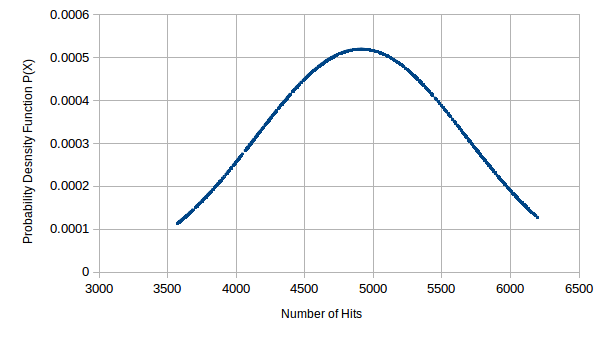
\includegraphics{call_hits_normal_distribution.png}
	\caption{Normal distribution plot of the number of hits for calls made}
	\label{exp2_fig1}
\end{figure}

\begin{figure}[h]
	\centering
	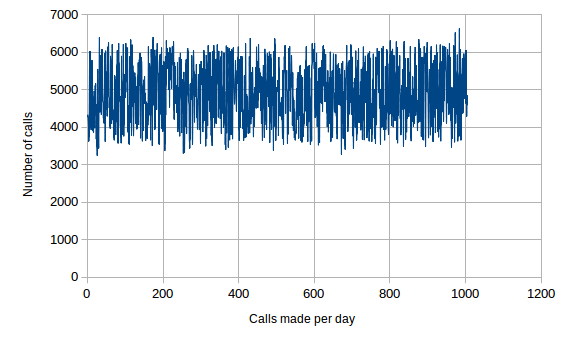
\includegraphics{time_series_plot_call_hit.png}
	\caption{Number of hits to call module as a time series plot}
	\label{exp2_fig2}
\end{figure}

\subsection{Analysis}
Plotted on the x-axis of figure \ref{exp2_fig1} is the number of calls made per day while on the y-axis is the probability density function (PDF) which is a dependent variable which responds to changes in X.
It is evident from figure \ref{exp2_fig1} that it follows a normal distribution with a mean of 4911.72 and a standard deviation of 767.76. Total number of calls 1 standard deviation to the left of the mean is considered below the mean that situation is considered bad anything below 2 standard deviations to the left of the mean is considered extreme. Figure \ref{exp2_fig2} shows the number of calls made per day over the past 1000 days as a time-series plot. A time-series plot is used for predicting and forecasting future events based on a previously observed pattern. It is evident that there were sharp drops in the total number of calls in between day 0 and day 50. These are considered outliers or extreme situation which is obviously 2 standard deviations to the left of the mean.

\section{Experiment 3: Workload predication}
The workload prediction problem comprises of ETL application workload and disk space availability predictions. The results from each of these experiments are presented in the subsequent sections. These predictions were framed as a supervised learning regression problem for the following reasons.

\begin{itemize}
	\item All the variables are continuous numeric and not category.
	\item There is a linear relationship between predictors and predictants or input and response.
	\item All the predictors are independent of each other.
	\item Data is free of missing values and outliers.
\end{itemize}

\subsection{ETL workload prediction}
\subsubsection{Aims}
The aim of this experiment is to test whether supervised regression models could be used to predict the future performance of an application based on continuous input variables. 

\subsubsection{Procedure}

\begin{itemize}
	\item 
\end{itemize}

\subsubsection{Result} 
The results for predicting the future performance of the ETL application is presented in Tables \ref{workloadPredDesc}, \ref{regresModelEval100} \& \ref{actualPred100} and illustrated in Figures \ref{fig_workloadPred100} and \ref{fig_workloadPred200}. Plotted on the x-axis is the running time and on the y-axis is the through put per second. The y-axis is the output/response we want to predict.

\begin{table}[h!]
	\centering
	\begin{tabular}{|l|l|l|l|}
		\hline
		\textbf{Metric} & \textbf{Payload} & \textbf{RunningTime} & \textbf{Throughput/sec} \\ \hline
		
				count  &  287.000000 &  287.000000 &     287.000000 \\ \hline
				mean &  89255.627178 &   52.613240  &   1827.247387 \\ \hline
				std &    3692.565405 &   12.841975 &     563.078152 \\ \hline
				min &   83076.000000 &   30.000000  &   1099.000000 \\ \hline
				25\%  &  85222.000000  &  40.000000 &    1427.000000 \\ \hline
				50\%  &  90167.000000 &   56.000000 &    1547.000000 \\ \hline
				75\%  &  92334.000000 &   63.000000  &   2296.000000 \\ \hline
				max  &  93655.000000  &  82.000000   &  3100.000000 \\ \hline

	\end{tabular}
	\caption{Workload prediction statistical metrics}
	\label{workloadPredDesc}
\end{table}


\begin{table}[h!]
	\centering
	\begin{tabular}{|l|l|l|}
		\hline
		\textbf{Metric} & \textbf{Value} \\ \hline
		Mean absoluate error (MAE):  &  3.21106048906 \\ \hline
		Mean squared error (MAE):   &  15.9477899498 \\ \hline
		Root mean squared error (RMSE):   &  3.99346841102 \\ \hline
		Constant/Intercept  &  92.54785537643912 \\ \hline
		Slope/coefficient  &  -0.02192117\\ \hline
	\end{tabular}
	\caption{Model evaluation and accuracy}
	\label{regresModelEval100}
\end{table}
\pagebreak

$$ 
Y = \beta o + \beta1X + \epsilon 
$$
$$ 
Y = -0.022x + 92.55 + 3.99
$$

\begin{center}
 \textbf{Univariate linear regression model for future workload prediction}
\end{center}


\begin{figure}[h]
	\centering
	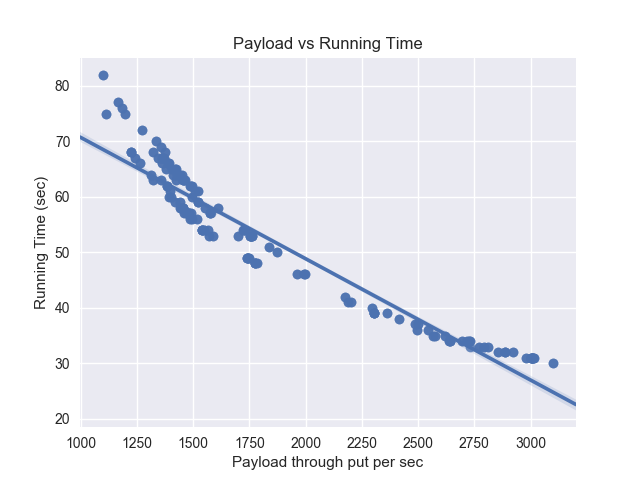
\includegraphics{workloadPrediction100.png}
	\caption{Workload prediction on actual values}
	\label{fig_workloadPred100}
\end{figure}


\begin{table}[h!]
	\centering
	\begin{tabular}{|l|l|l|l|}
		\hline
		\textbf{No} &     \textbf{Actual} &   \textbf{Predicted} &   \textbf{Through put per sec} \\ \hline
		0   &    54 & 58.263138   &              1564 \\ \hline
		1   &   67 & 62.537767       &          1369 \\ \hline
		2   &   62 & 62.230871     &            1383 \\ \hline
		3   &    31 & 27.266597     &            2978 \\ \hline
		4   &    38 & 39.564376    &             2417 \\ \hline
		5   &    60 & 61.792447    &             1403 \\ \hline
		6   &    39 & 42.041469    &             2304 \\ \hline
	\end{tabular}
	\caption{Actual and predicted workload}
	\label{actualPred100}
\end{table}


\begin{figure}[h]
	\centering
	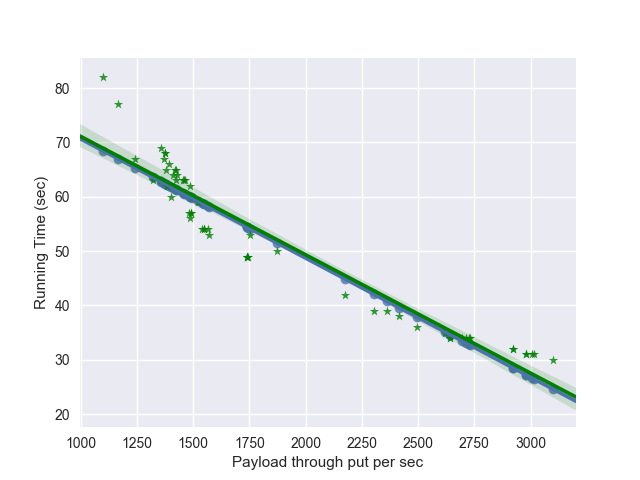
\includegraphics{workloadActualAndPredicted.png}
	\caption{Graph of actual and predicted workload}
	\label{fig_workloadPred200}
\end{figure}


\subsubsection{Analysis}
We can see from the results that the mean values for the payload, total running time and through put/sec is calculated as 89255.63, 52.61 and 1827.25 respectively. This values represent the an average across the observed sample size of 287 records which was used for the test and prediction sample. A standard deviation of 3692.57, 12.84 and 563.08 was also obtained for each of these features respectively.


\subsubsection{Model Evaluation}
The accuracy of the model was evaluated using Root Mean Squared Error (RMSE), Mean Absolute Error (MAE) and Mean Squared Error (MSE). The RMSE value of $3.993 \approx 4$. This implies that our error is less than 7.6 8\% of the observed mean value of 52.61. A less than 10\% error is evidence of a good regression model.


\section{Experiment 4: Anomaly detection}
This

\subsection{Result} 

\subsection{Analysis}


\chapter{\textbf{Conclusion and Discussion}}


\bibliographystyle{agsm}
\bibliography{thesis}

\end{document}